\section{Livelits by Example}\label{sec:case-studies}


In this section, we will detail the livelits mechanism by way of  
two domain-specific case studies:
a course grade assignment case study in Sec.~\ref{sec:live-grading}
and an image transformation case study in Sec.~\ref{sec:image-transformation}.
% We also briefly mention several other examples in Sec.~\ref{sec:additional-examples}.\todo{do we?}{}
These case studies have been implemented
in Hazel, a browser-based live programming environment for a dialect of Elm. 
Elm is an industrial pure typed functional language in the
ML family used for client-side web development. 
We assume basic familiarity with ML.

\subsection{Case Study: Grading with Livelits}\label{sec:live-grading}
Consider this familiar scenario: an instructor needs
(1) to record numeric grades for various assignments and exams, and
(2) to visualize and perform various computations with these numeric grades
in order ultimately to assign final letter grades.
(In fact, this case study is not contrived: one author is using Hazel to compute grades this semester.)

The most common end-user application for this task is the spreadsheet, because 
it allows the instructor to record grades using a natural tabular interface,
visualize this data in one of a finite number of plot styles, 
and perform basic computations,
with results updated live.
However, these affordances are limited. 
It is difficult to package up common operations 
into reusable libraries, interact with the data using domain-specific visualizations,
and perform complex, unanticipated operations 
(e.g. preparing the data in an idiosyncratic format demanded by the university's grading system).

General-purpose programming languages 
can handle these scenarios, but users 
lose the ability to receive live feedback and  
directly manipulate data and visualizations in the editor.

Livelits are able to address this tension.
Fig.~\ref{fig:grading}(c)\todo{sublabels} shows a Hazel program where 
the instructor alternates between programmatic and direct manipulation in several situations.

First, the instructor defines a value \li{grades} 
that records the grades for each student using a livelit, \li{\$dataframe}, 
that implements a tabular user interface. The formula bar 
allows the selected cell to be filled with an arbitrary Hazel expression. 
For the sake of demonstration, we show a cell that has been filled using another livelit, 
\li{\$slider}, in combination with symbolic manipulation.\todo{do this?}{}
The table itself displays not the expression itself but rather its value, just as in a spreadsheet.

Next, the instructor computes \li{averages} 
for each student by applying \li{compute_averages}, a helper function 
defined in a library  (not shown) shared between multiple courses.

Next, the instructor wants to ``eyeball'' reasonable \li{cutoffs} between letter grades 
by directly manipulating a domain-specific livelit, \li{\$grade_cutoffs}, that provides draggable ``paddles'' 
superimposed on a live visualization of the distribution of \li{averages}, which is provided as a livelit parameter.
% The value of \li{cutoffs} is a labeled 4-tuple containing each cut-off. 

Finally, 
the instructor programmatically assigns grades to students 
based on these \li{cutoffs} 
by calling \li{assign_grades} 
and \li{format_for_university},
again shared functions.

\subsection{Livelit Expansion}\label{sec:livelit-expansion}
Livelit invocations 
expand to expressions.
For example, the expansion of Fig.~\ref{fig:grading}(c) is:

\begin{lstlisting}[xleftmargin=0.2cm]
let grades = Dataframe (
  ["A1", "A2", "A3", "Midterm", "Final"],
  [("Alice", [24. +. 36. +. 33., 
              92., 83.5, 95., 88.]),
   ("Bob", [61., 64., 98., 70., 85.]),
   ("Ciri", [75., 81., 73., 82., 79.]),
   (* ... *) ]) in
let averages = compute_averages grades weights in
let cutoffs = (.A 90., .B 80., .C 70., .D 60.) in
format_for_university 
  (assign_grades averages cutoffs)
\end{lstlisting}

The client can inspect this expansion in Hazel via a toggle (not shown).
Ideally, however, reasoning about types and binding
should not require the client to inspect the expansion 
nor the livelit implementation (which specifies the expansion logic 
as we will describe in Sec.~\ref{sec:livelit-definitions}).
After all, function clients do not need to look inside
function bodies to reason about types and binding.
Instead, in the words of \citet{DBLP:conf/ifip/Reynolds83},
``type structure is a syntactic discipline for maintaining levels of abstraction''.
Livelits maintain this discipline by
several means, described next in Sec.~\ref{sec:expansion-typing}-\ref{sec:hygiene}.

\subsubsection{Expansion Typing} 
\label{sec:expansion-typing}
To support abstract reasoning about the type of the expansion,
livelit definitions declare an \emph{expansion type}.
The declarations of the livelits in Fig.~\ref{fig:grading},
eliding their implementations, are:
\begin{lstlisting}[numbers=none,xleftmargin=0cm]
livelit $dataframe at Dataframe {...}
livelit $grade_cutoffs(averages: List(Float)) at 
  (.A Float, .B Float, .C Float, .D Float) {...}
livelit $slider (min: Int) (max: Int) at Int {...}
\end{lstlisting}
The expansion type of \li{\$dataframe} is \li{Dataframe},
which classifies tabular floating point data together with string row and column names (see the expansion above).
The expansion type of \li{\$grade_cutoffs} is a labeled product of grade cutoffs (field labels are written \li{.label}
rather than \li{label:} in Hazel).
Hazel displays the information in the livelit declaration when the cursor is on the livelit's name,
just as it displays typing information in other situations (not shown).\todo{cite HATRA}{}

\subsection{Compositionality}\label{sec:splicing-and-parameterization}
Livelits are compositional: they can work with sub-expressions  
in the form of parameters and splices.

\subsubsection{Parameters}\label{sec:parameterization} 
Livelit can declare a finite number of parameters of specified types. 
For example, \li{\$grade_cutoffs} above declares one parameter,
the averages to be plotted, of type \li{List(Float)}.
Parameters are applied  
using function application notation 
as seen in Fig.~\ref{fig:grading}(c) or 
using the pipelining (i.e. reverse function application) operators, \li{<|} and \li{|>}, 
which allow multiple livelits to form dataflows (not shown).

Livelit abbreviations can partially apply parameters. For example, 
we can partially apply the first parameter of \li{\$slider} to define a parameterized unsigned slider livelit:
\begin{lstlisting}[numbers=none,xleftmargin=0cm]
let $uslider = $slider 0 in ...
\end{lstlisting}
Only livelits with no remaining parameters can be invoked, 
so writing \li{\$uslider} in expression position will display as a ``missing livelit parameter'' error.%
\footnote{\label{footnote:typing}In Hazel, erroneous expressions 
are automatically placed inside holes so that they do not prevent other parts of the program from evaluating
\cite{HazelnutLive}.}


\begin{figure*}
  \begin{center}
    \begin{subfigure}[t]{0.5\textwidth}
      \centering
      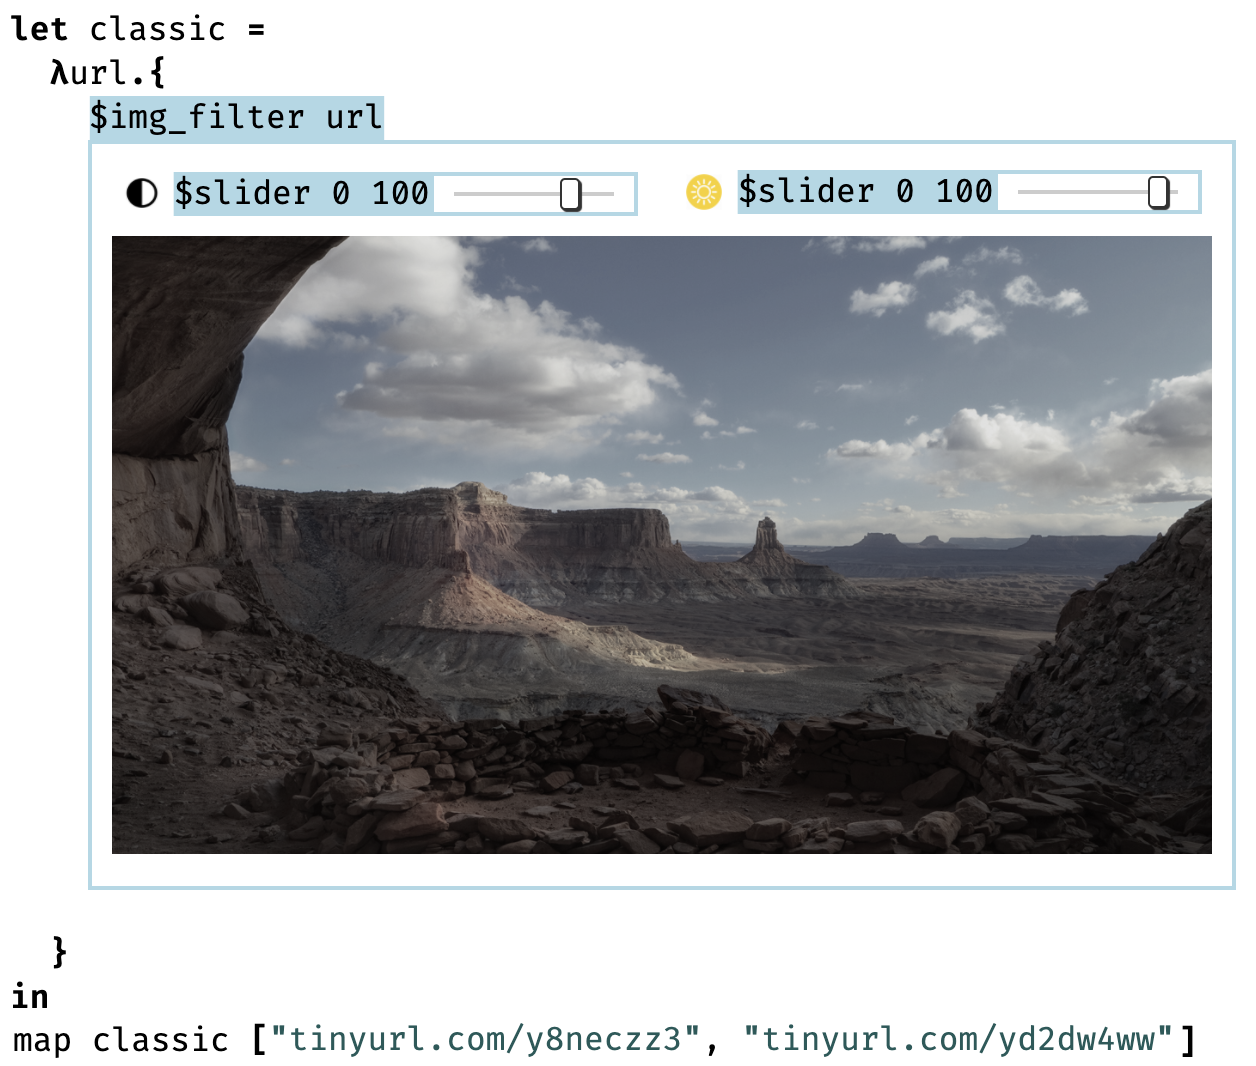
\includegraphics[width=15pc]{img-filter-1.png}
      \caption{}
    \end{subfigure}\begin{subfigure}[t]{0.5\textwidth}
      \centering
      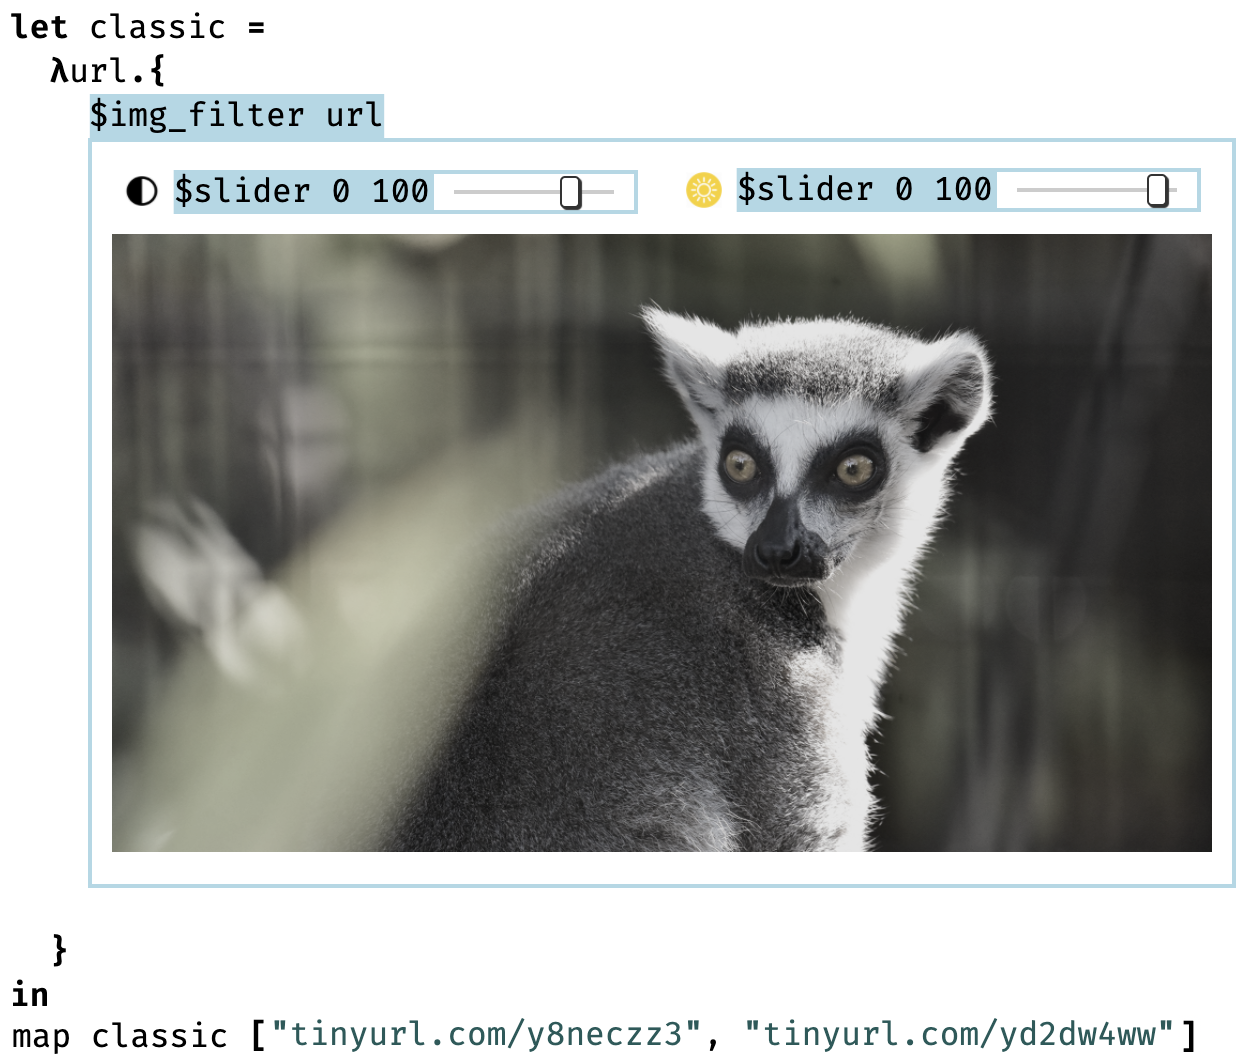
\includegraphics[width=15pc]{img-filter-2.png}
      \caption{}
    \end{subfigure}
  \end{center}
  \caption{Case Study: Image Transformation. The image shown is determined based on the selected closure.}
  \label{fig:img-transformation}
\end{figure*}


\subsubsection{Splices}\label{sec:splices}
Spliced expressions, or \emph{splices}, appear directly inside the livelit GUI.
Splices can be filled with Hazel expressions of any form, including other livelit invocations.
For example, each cell in the \li{\$dataframe} GUI in Fig.~\ref{fig:grading}
has a corresponding splice. The formula bar at the top 
allows the user to edit the splice corresponding to the selected cell,
and all of Hazel's editing affordances are available when the client does so.
% Not all splices necessarily appear in the GUI.
Unlike parameters, the number of splices can change 
as the user interacts with the livelit, e.g. when changing the number of rows or columns in a \li{\$dataframe}.
% The cell itself displays the live value of the spliced expression---
% (we return to live evaluation in Sec.~\ref{sec:live-evaluation} below.

The livelit provides an expected type for each splice when it is created.
For example, the splices for the row and column keys in Fig.~\ref{fig:grading}(c)\todo{go through subfigures}{} have expected type \li{String}, 
and the remaining cells have expected type \li{Float}.
Hazel surfaces and uses the expected type when the cursor is in the splice.\todo{cite HATRA paper}{}
% If an expression of invalid type is entered, it will display in an error hole as usual,
% and in Hazel this will not prevent evaluation of other expressions (see Footnote \ref{footnote:typing}).

% Unlike parameters, the number of splices is not fixed in the livelit declaration. Splices can be created,
% deleted, and filled through user interaction with the livelit. For example, clicking the \li{+} buttons
% in Fig.~\ref{fig:grading} will create new rows or columns, which will in turn generate new splices.

\subsubsection{Hygienic Composition}\label{sec:hygiene}
 

Ensuring that clients can reason about binding while leaving expansions
 invisible 
 requires a hygiene discipline that enforces \emph{capture avoidance}
and \emph{context independence} \cite{TLMs}\todo{cite michael hygiene paper}.

\textbf{Capture Avoidance.}
Splices and parameters can appear anywhere in the expansion. 
This becomes problematic when
they appear under a binder, e.g. in the body of a function or \li{let} binding.
Na\"ively, this could cause inadvertent capture of the bound variable by a free variable
in the parameter or splice. For example, consider a livelit that generates an expansion
of the following seemingly innocuous form:
\begin{lstlisting}[numbers=none]
let len = strlen <splice1> in
Some (<splice2> + len)
\end{lstlisting}
Here, \li{<splice2>} appears under the binding of \li{len}. If the client has filled
\li{<splice2>} with an expression that refers to a client-side binding of \li{len},
these references would na\"ively be captured. This would not occur in \li{<splice1>}, 
because the \li{let} is not recursive.
This breaks abstraction and is notoriously difficult to debug,
both for the livelit provider, who has no way to predict which variables a client will use,
 and the client, who does not know which variables the provider used.

To avoid this situation, parameters and splices are placed in the expansion
in a capture-avoiding manner: variables in splices
always refer to the bindings visible to the client, 
rather than bindings that are hidden inside the expansion.
We discuss how this is implemented in Sec.~\ref{sec:expansion}.
% This is implemented by alpha-renaming bindings internal to the expansion as necessary.
% (We discuss potentially relaxed variations of this hygiene discipline in Sec.~\ref{sec:discussion}.)

\textbf{Context Independence.}
The example expansion above used a library function, \li{strlen}.
Na\"ively, this expansion would break if placed 
in client contexts where \li{strlen} is not bound, or bound to 
an unexpected value.
To avoid requiring clients to determine and satisfy these invisible 
dependencies, the livelits mechanism enforces \emph{context independence}:
generated expansions are valid in any context. Dependencies are bound 
relative to the livelit definition site (see Sec.~\ref{sec:expansion}).

\subsection{Live Evaluation}\label{sec:live-evaluation}
Livelits have the ability to evaluate a splice or a parameter 
in order to provide better feedback about run-time behavior to the client.
The \li{\$dataframe} livelit uses this facility to display
the evaluation result for each cell, like a spreadsheet.
The \li{\$grade_cutoffs} livelit uses this facility to plot the grades, which were 
passed in as a parameter, on the number line.

\subsubsection{Closure Collection} The subtlety is that 
evaluation in Hazel is defined for closed expressions as usual,
but parameters and splices can be open, i.e. refer to surrounding variables. 
To provide a environment that binds these variables, 
Hazel performs \textbf{closure collection} in two phases.

In the first phase, \emph{proto-closure collection}, 
Hazel replaces each livelit with a uniquely numbered hole and then evaluates the program 
using the semantics for evaluating programs with holes developed by \citet{HazelnutLive}.
Evaluation proceeds around these holes, producing a result containing 
corresponding hole closures, i.e. holes with environments.

For example, there is one closure for \li{\$dataframe} in Fig.~\ref{fig:grading}.
It contains the value of \li{q1max}\todo{what?}{} and the other variables in scope. 
These values can be used to evaluate 
splices that use the corresponding variables, such as the cell selected in Fig.~\ref{fig:grading}(c). 

Similarly, the closure for \li{\$grade_cutoffs} in Fig.~\ref{fig:grading} includes 
the necessary \li{averages} variable, but 
its value depends on \li{grades}, which is determined by \li{\$dataframe}. 
If we stop after proto-closure collection,
then no useful value will be available:
the result will be \emph{indeterminate}, because \li{\$dataframe} has been replaced with a hole \cite{HazelnutLive}.
For this reason, there is a second phase of closure collection, called \emph{closure resumption}, 
where any livelit holes that appear
in the collected livelit closures are \emph{resumed}, i.e. the expansion is generated
(in this case, for the \li{\$dataframe} livelit) and evaluation resumes.
% Livelit expansions do not contain livelits, so no subsequent expansion / resumption phases are necessary.

% Hazel does not need to evaluate the program multiple times in order to support live closure collection
% as well as the usual live evaluation services it offers, because the final evaluation result 
% can also be determined by resumption.
% (We discuss how to address subtleties that arise 
% in the presence of non-commutative side effects in Sec.~\ref{sec:calculus-closure-collection}.)

\subsubsection{Indeterminate Results}
Even after resumption, some elements of the closure may remain indeterminate, e.g. due to holes that 
are not filled with livelits. 
When a livelit requests an evaluation result, it must be able to handle these indeterminate results.
For example, if there were missing grades,
then \li{\$grade_cutoffs} would have degraded functionality: 
it would display only the list elements that are values on the timeline, skipping indeterminate elements.
We will return to how this occurs in Sec.~\ref{sec:live-evaluation-def}.



\subsubsection{Case Study: Live Photo Filters}\label{sec:image-transformation}
\todo{revise this once we have final figure}{}
Closure collection can produce multiple closures when, for example, 
a livelit appears inside a function applied multiple times. 
Our next case study, in the photography domain,
demonstrates how Hazel handle this situation, and 
the workflow it enables. 

We interviewed a photographer 
who described a typical workflow: 
they use the Lightroom application to 
apply a set of adjustments and filters 
across all photos in a collection before making 
individual adjustments. 
Many photographers do this one photo at a time,
though this photographer had recently learned how to
use Lightroom's saved presets to 
apply adjustments to multiple photos at once.
However, they remained dissatisfied by the workflow.
They wanted to be able to see how the shared settings affected 
multiple photos as they tweaked them, without having to 
save and apply the preset repeatedly.
They also wanted to be able to change the shared settings
even after making certain individual adjustments.
They also expressed interest in defining parameterized 
presets, and in automating the process of 
posting sets to a website and social media. 

% For our next case study, we 
% developed a library of 
% image transformation livelits, 
% motivated by a desire to automate 



% The livelits we have considered so far generate simple values.

Motivated by this interview, 
we prototyped a collection of image transformation livelits.
One of these, \li{\$something} is demonstrated in Fig.~\ref{fig:img-transformation},
within a function, \li{classic_look}, that serveas as a ``preset'' that is 
mapped over a list of images (loaded by URL) at the bottom of the figure. 
% We show two for space reasons.

...\todo{finalize?}{}
This livelit takes 
a URL to an image as a parameter, and contains two splices of type \li{Int},
one to adjust the contrast, and the other to adjust the brightness.
In this example, we have filled those splices with a \li{\$slider}, but 
as above we could enter any expression of type \li{Int}, e.g. 
an arithmetic expression or a variable. 
The livelit shows a live preview of the transformed image.
The expansion generates the necessary calls to an image processing library, 
not shown.

Because the livelit appears inside a function applied (by \li{map}) twice, 
there are now two closures associated with the livelit. 
Rather than disabling live evaluation in situations like 
this, Hazel instead allows the programmer to select between the closures when 
the cursor is on the livelit expression via a simple sidebar toggle. 
This causes the view to change as shown in ...\todo{todo}{}
The live feedback is based on the selected closure.
This makes it easy to see how the image filter being designed here will affect a
number of example images by quickly toggling between closures. 
The underlying expansion remains abstract, i.e. it refers to the image via the \li{url} variable.

We showed this and similar examples to the photographer we had interviewed. 
They expressed substantial interest in this approach despite having only 
limited programming experience (with Python). They made the fair point that it 
would take substantial effort to match Lightroom's breadth of filters and effects, 
but with sustained effort, they agreed that this approach could be more powerful than 
Lightroom's point-and-click interface while retaining many of its benefits (specifically
mentioning the graphical sliders). Although this was only a single interview,
it is consistent with the body of evidence summarized in Sec.~\ref{sec:background}.

% \subsection{Additional Examples}\label{sec:additional-examples}
% It would be nice to have a gallery-style figure and a brief overview of some other case studies
% and how they exercise the novel features of the livelits mechanism. Maybe some statistics on how
% many lines of code it took.

% Ideas:
% \begin{itemize}
%   \item derivation trees like Joomy's system (\url{https://joom.github.io/proof-tree-builder/src/})
% \end{itemize}